\vspace{-0.25in}
\section{Experiment}
\vspace{-0.05in}
\subsection{Predictive Performance}
\vspace{-0.1in}
%datasets
\begin{figure*}
	\centering
	\setlength\tabcolsep{0.01pt}
	\begin{tabular}[c]{cccc}
		\multicolumn{4}{c}{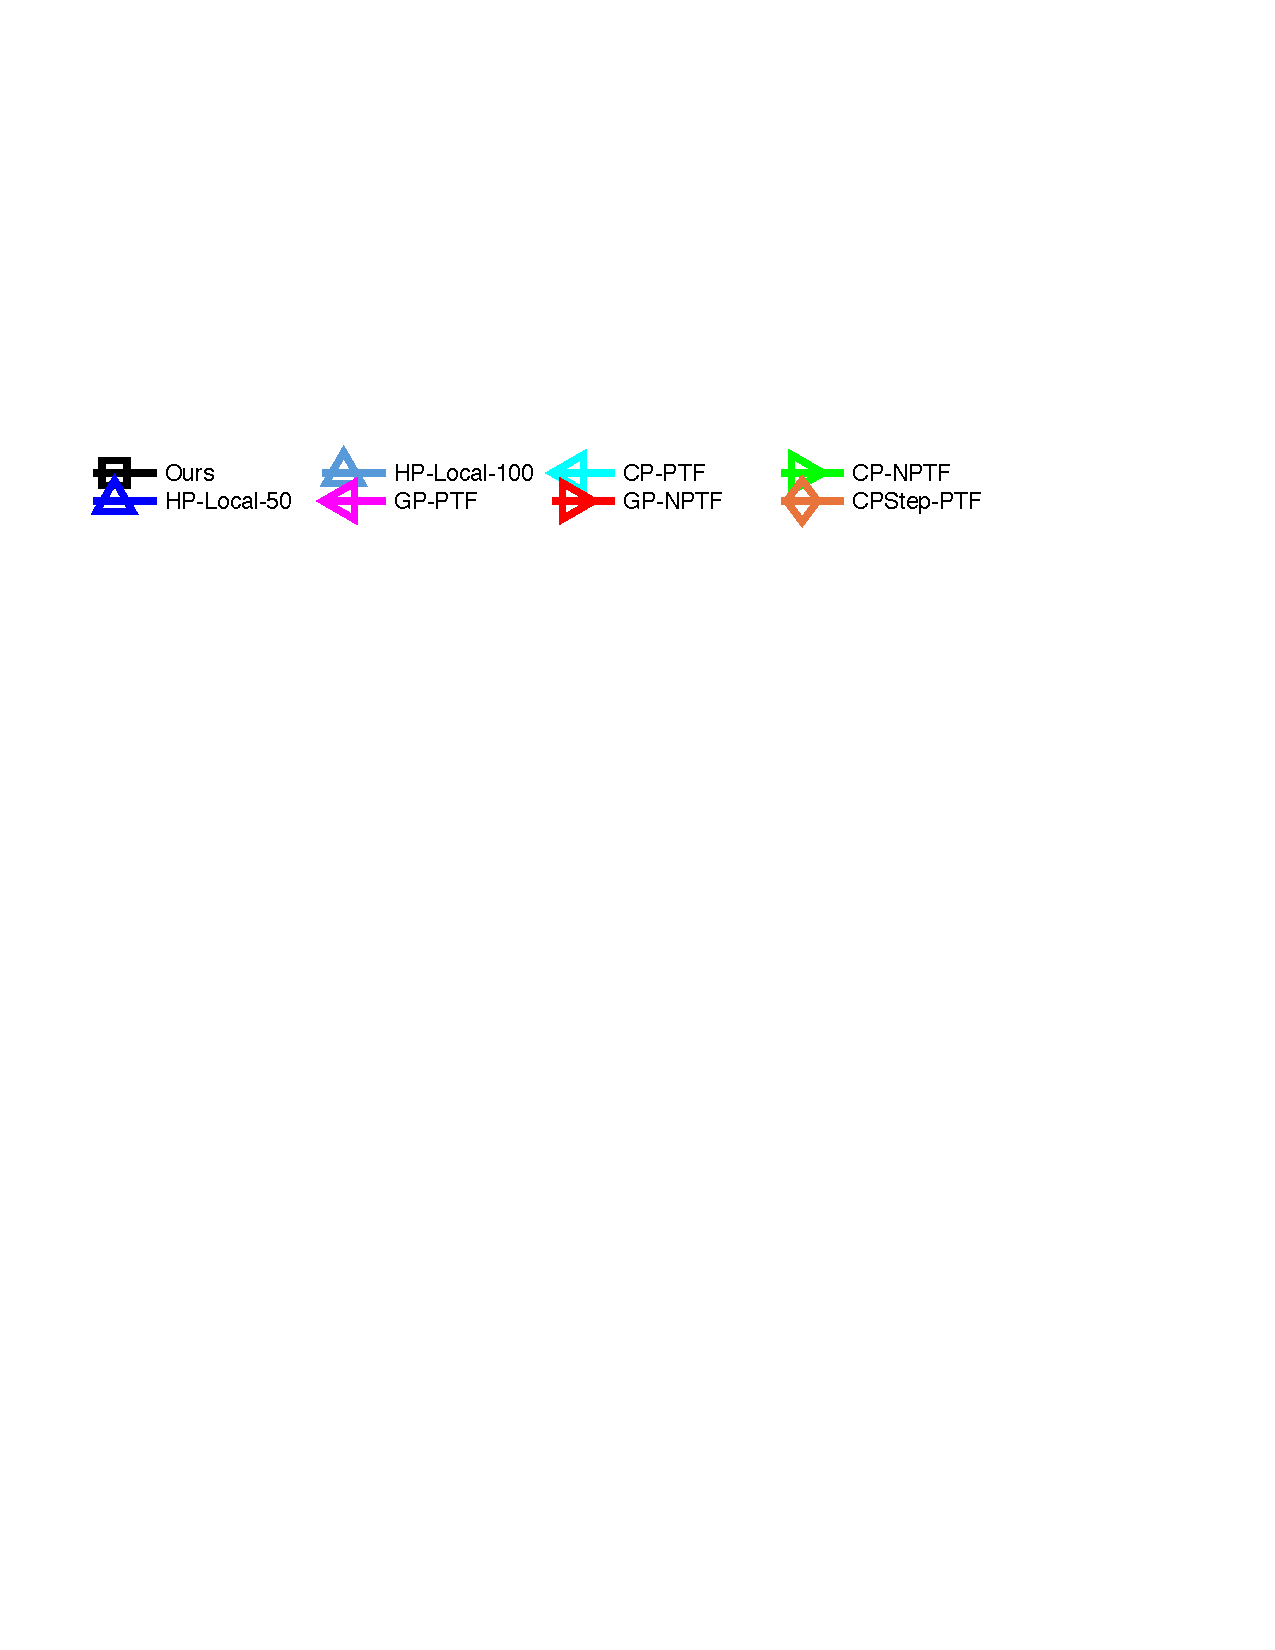
\includegraphics[width=0.618\textwidth]{./figs/ll_legend.pdf}}
		\\
		\begin{subfigure}[t]{0.25\textwidth}
			\centering
			%			\includegraphics[width=\textwidth]{./fig/burger_400_rmse.eps}
			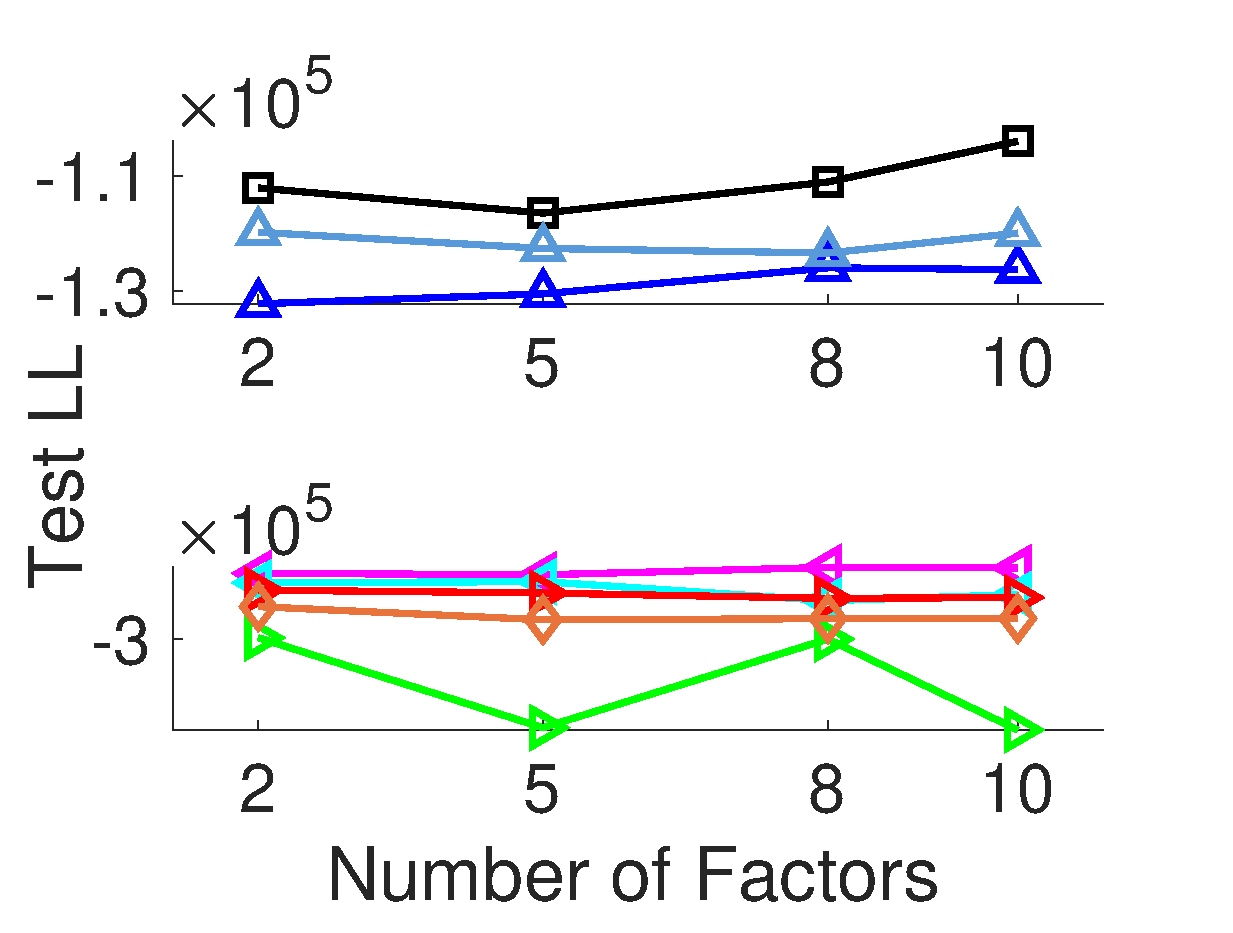
\includegraphics[width=\textwidth]{./figs/taobao_ll.eps}
			\caption{\textit{Taobao}}
		\end{subfigure} 
		&
		\begin{subfigure}[t]{0.25\textwidth}
			\centering
			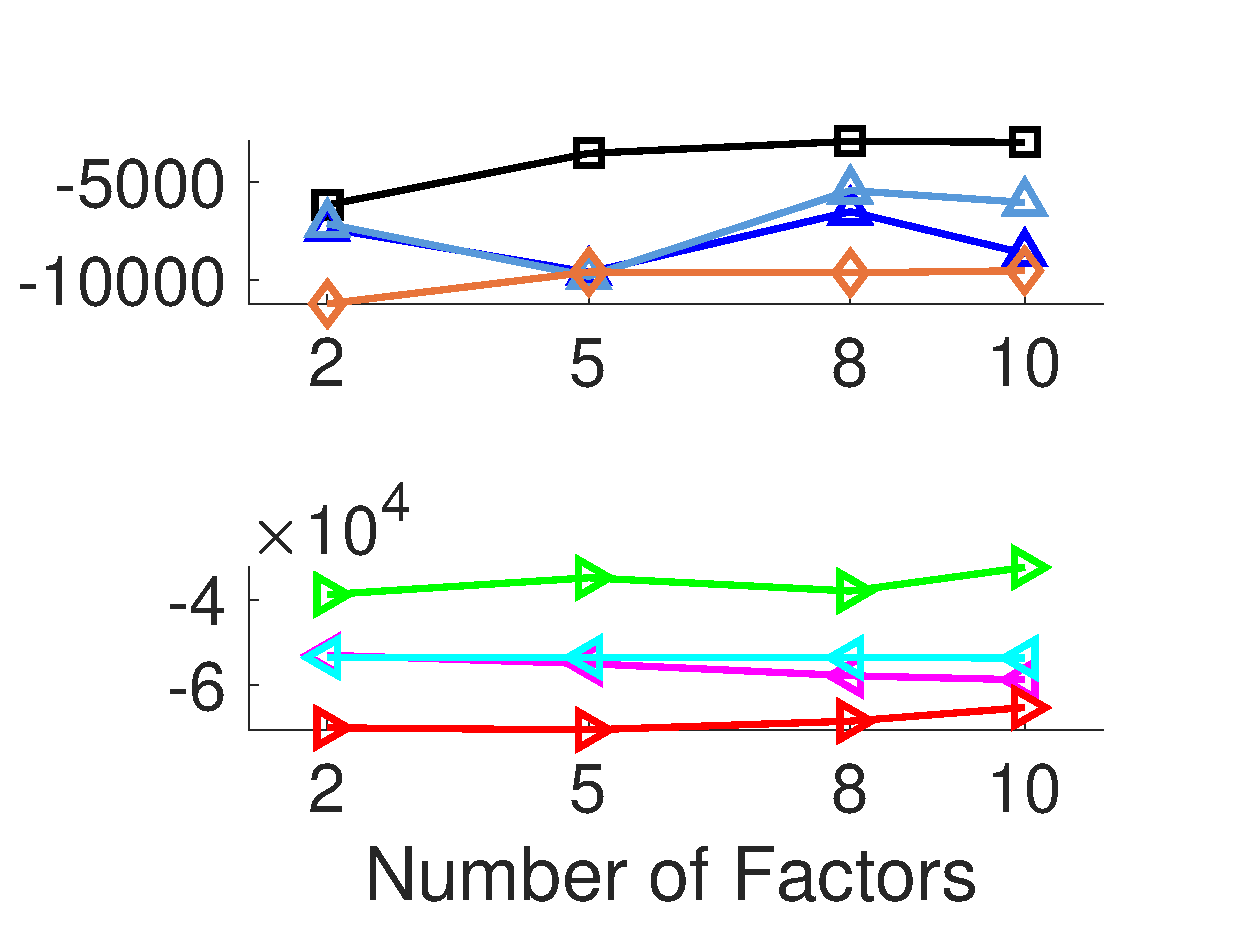
\includegraphics[width=\textwidth]{./figs/ufo_ll.eps}
			\caption{\textit{UFO}}
		\end{subfigure}
		&
		\begin{subfigure}[t]{0.25\textwidth}
			\centering
			%			\includegraphics[width=\textwidth]{./fig/heat_400_rmse.eps}
			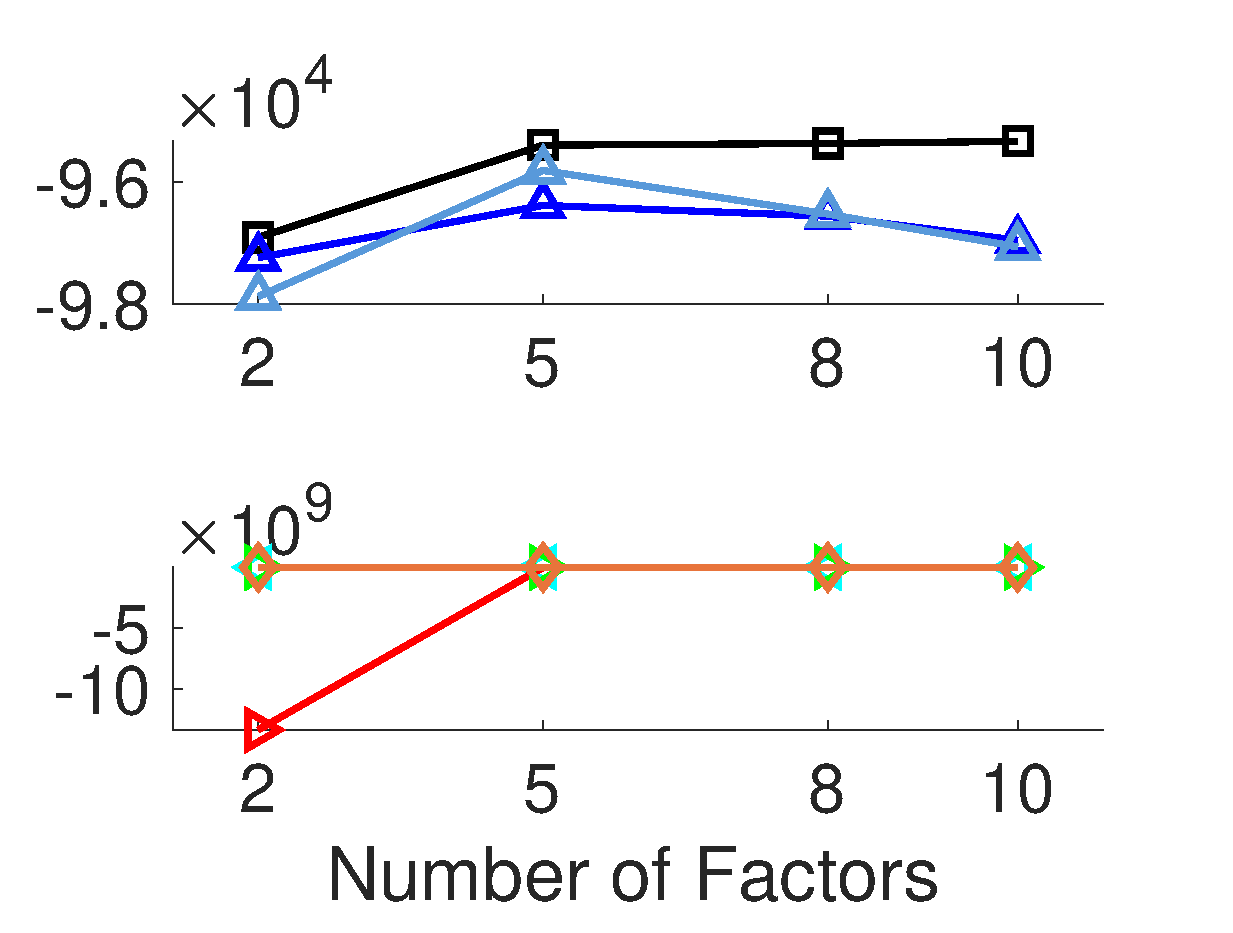
\includegraphics[width=\textwidth]{./figs/crash_ll.eps}
			\caption{\textit{Crash}}
		\end{subfigure} 
		&
		\begin{subfigure}[t]{0.25\textwidth}
			\centering
			%			\includegraphics[width=\textwidth]{./fig/heat_400_rmse.eps}
			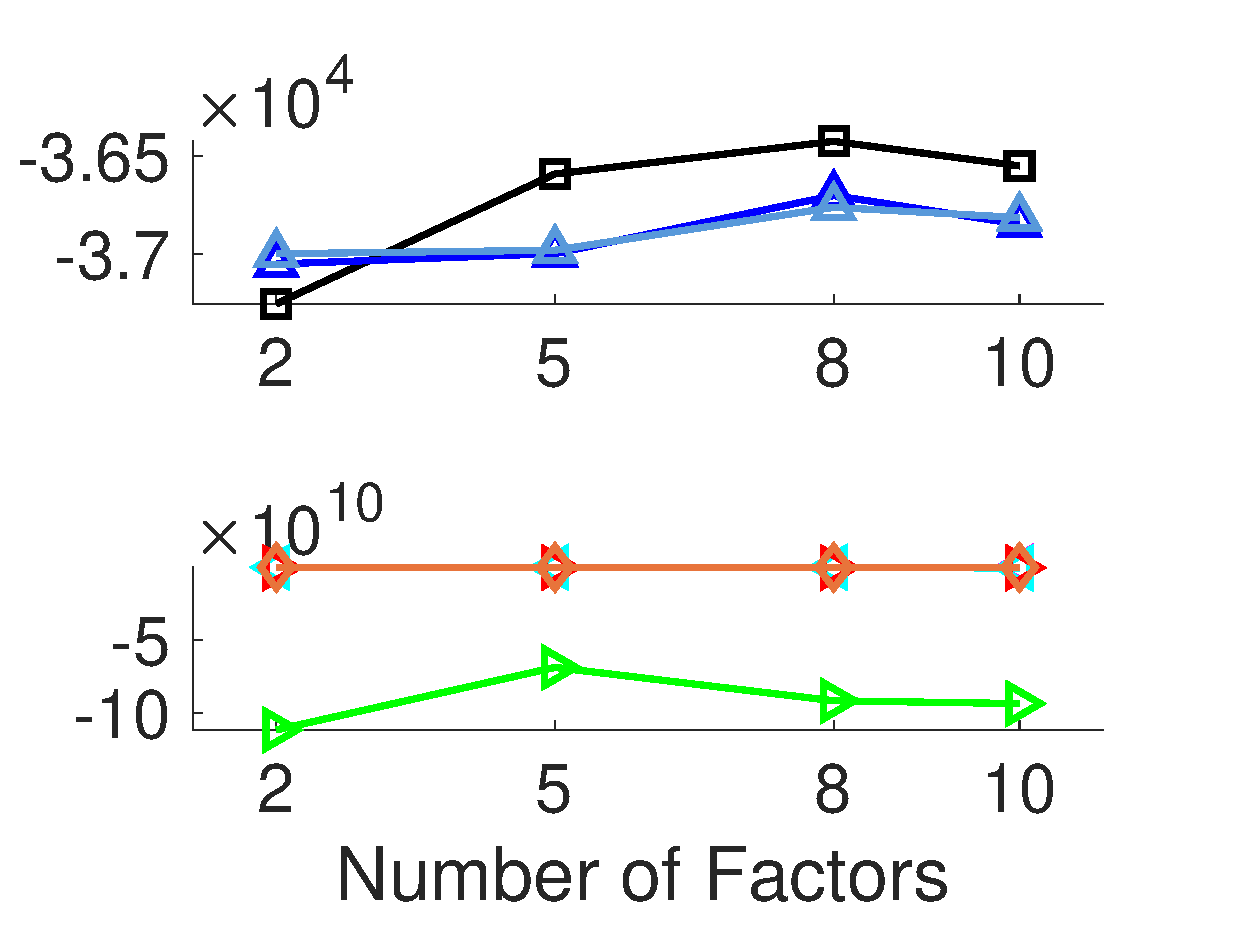
\includegraphics[width=\textwidth]{./figs/lastfm_ll.eps}
			\caption{\textit{LastFM}}
		\end{subfigure} \cmt{\\
		\begin{subfigure}[t]{0.25\linewidth}
			\centering
			%			\includegraphics[width=\textwidth]{./fig/burger_400_rmse.eps}
			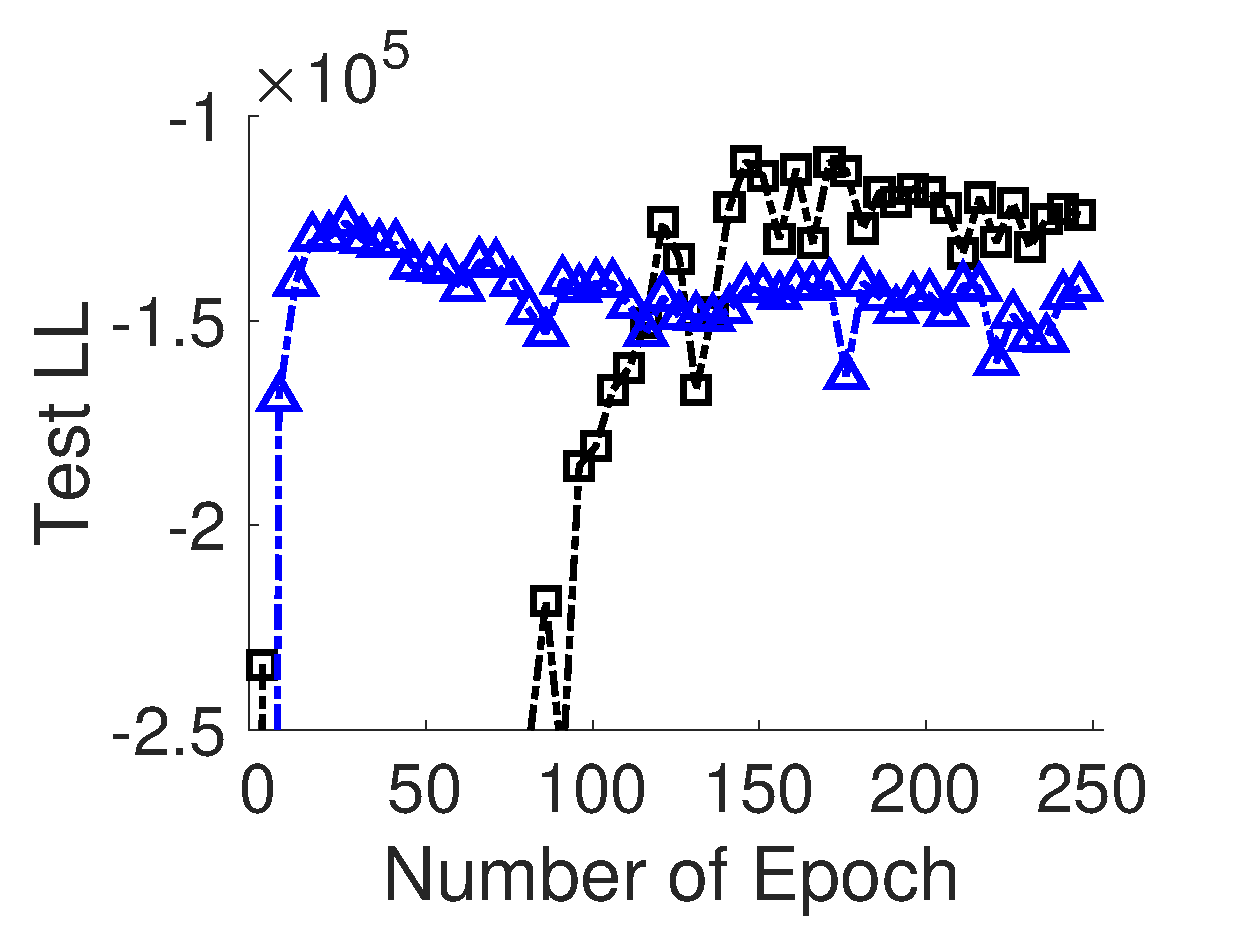
\includegraphics[width=\linewidth]{./figs/taobao_ll_epoch.eps}
			\caption{\textit{Taobao}}
		\end{subfigure} 
		&
		\begin{subfigure}[t]{0.25\linewidth}
			\centering
			%			\includegraphics[width=\textwidth]{./fig/burger_400_rmse.eps}
			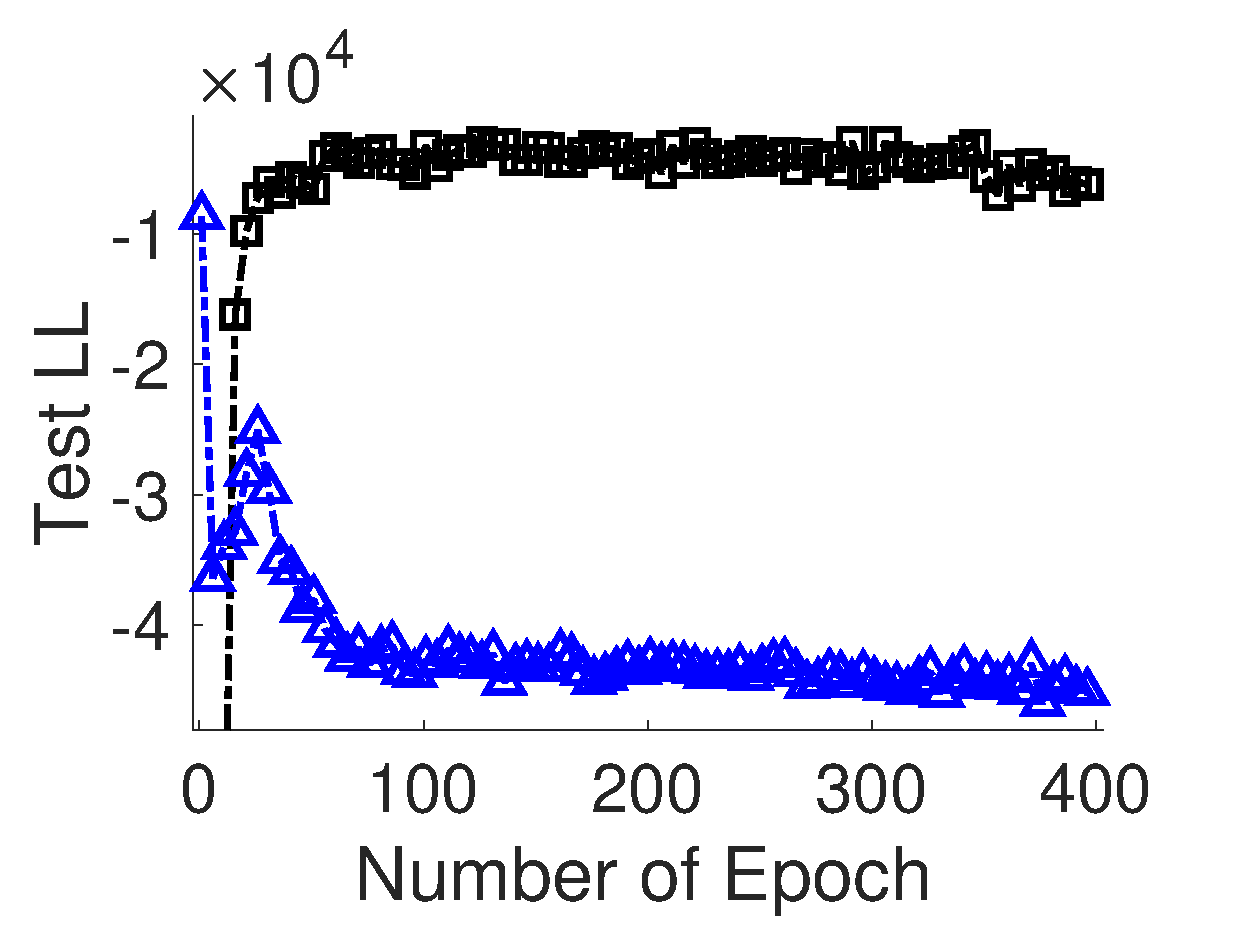
\includegraphics[width=\linewidth]{./figs/ufo_ll_epoch.eps}
			\caption{\textit{UFO}}
		\end{subfigure} 
		&
		\begin{subfigure}[t]{0.25\linewidth}
			\centering
			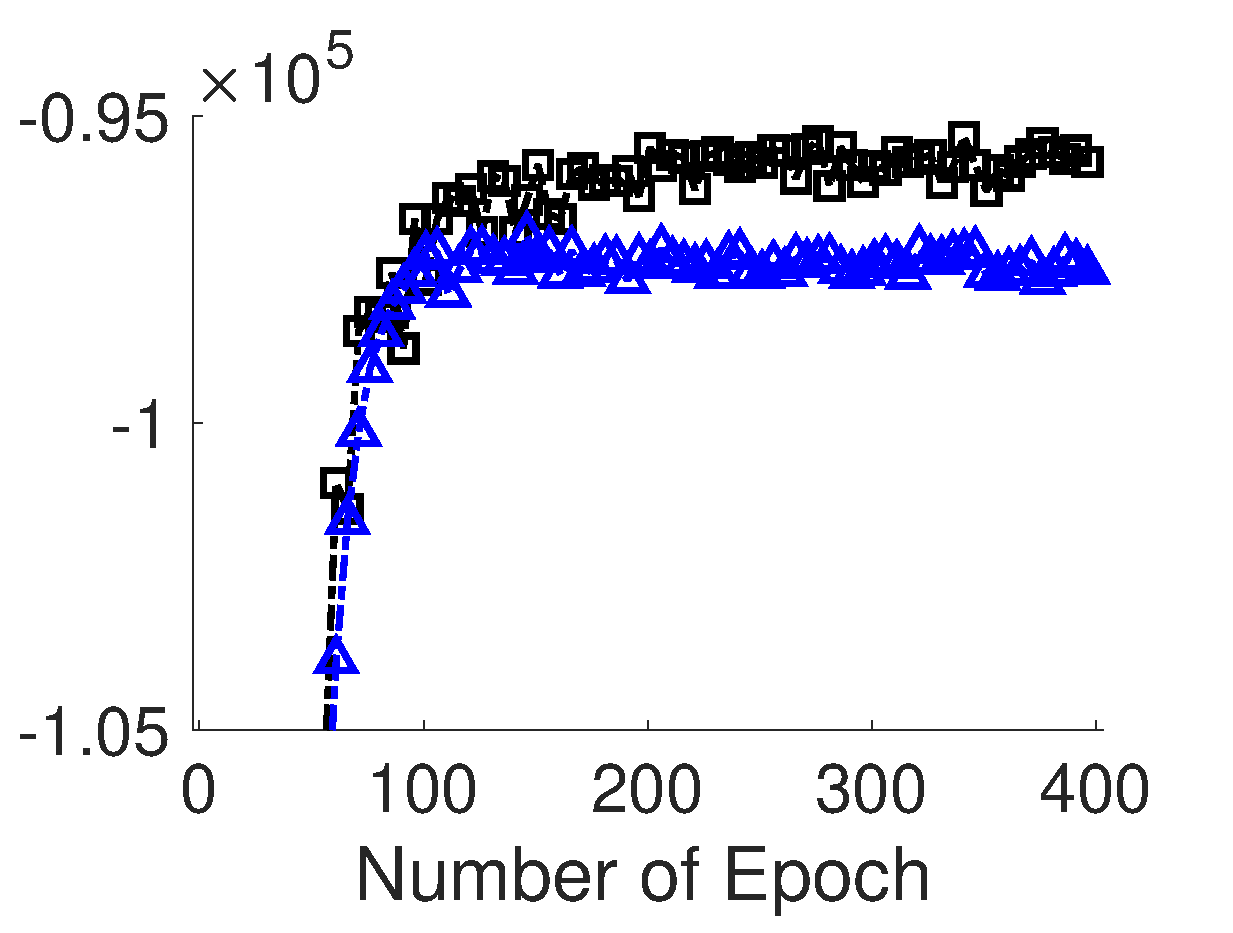
\includegraphics[width=\linewidth]{./figs/crash_ll_epoch.eps}
			\caption{\textit{Crash}}
		\end{subfigure}
		&
		\begin{subfigure}[t]{0.25\linewidth}
			\centering
			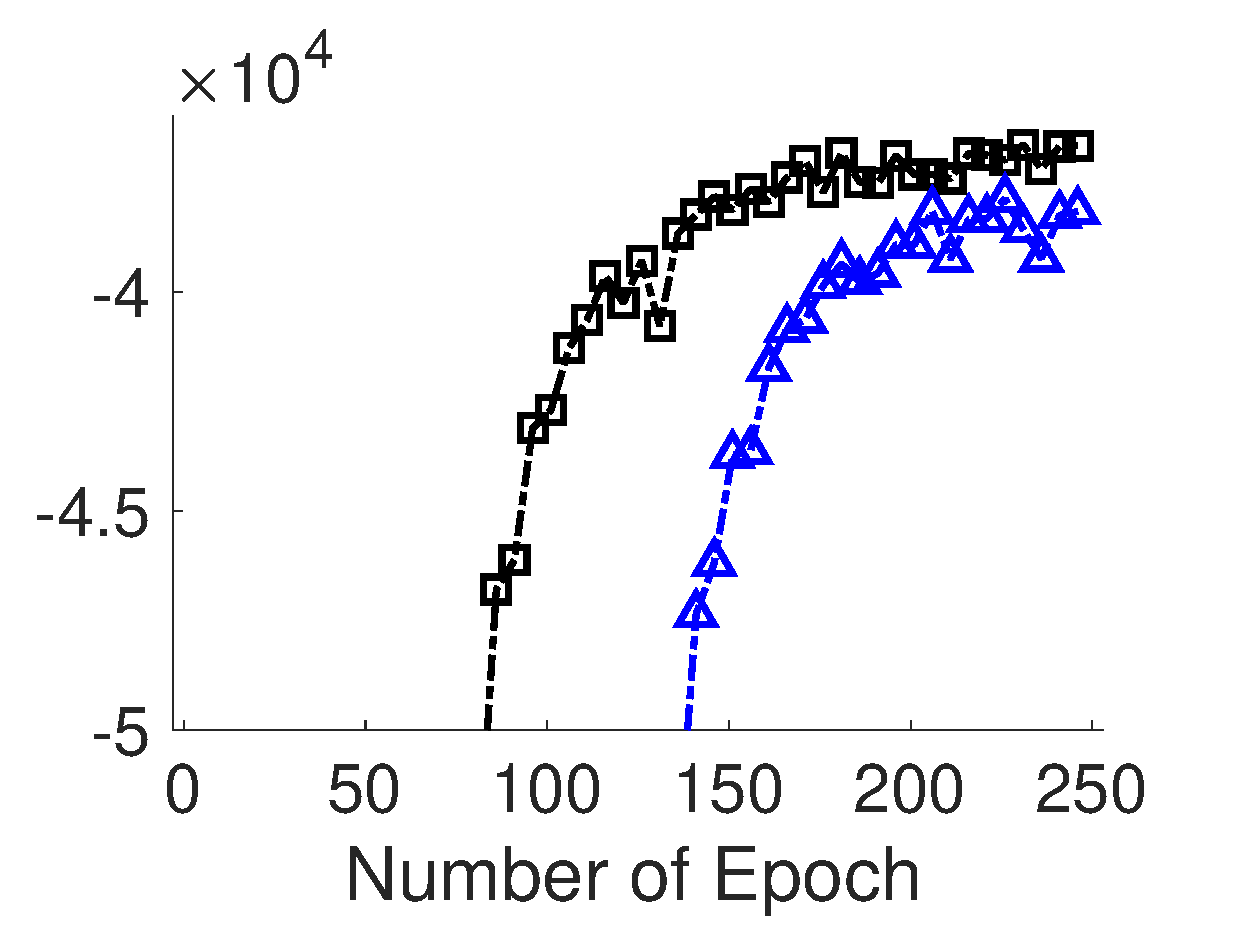
\includegraphics[width=\linewidth]{./figs/lastfm_ll_epoch.eps}
			\caption{\textit{LastFM}}
		\end{subfigure}
	}
	\end{tabular}
	\vspace{-0.1in}
	\caption{Test log likelihood on each dataset with different number of latent factors. HP-Local-\{50, 100\} means running HP-Local with window size $50$ and $100$. The sub-figures on the top include the results only for our method and HP-Local, except that in (b), CPStep-PTF is also included. All the remaining methods are shown in the bottom sub-figures and their performance are much worse. Note that the test log likelihoods of several baselines are very close on \textit{Crash} and  \textit{LastFM} and so their curves overlap. } 	
	\label{fig:test-ll}
	\vspace{-0.2in}
	%\vspace{-0.14in}
\end{figure*}
\textbf{Datasets}. We first examined the predictive performance of our approach on the following four real-world datasets.  (1) \textit{Taobao} (\url{https://tianchi.aliyun.com/dataset/dataDetail?dataId=53}), online shopping behaviours between 07/01/2015 and 11/30/2015 in the largest retail platforms of China. We extracted a $5$-mode tensor, of size $980 \times 274 \times  631 \times  58 \times  2$, which represents the interactions of  \textit{(user, seller, item, category, action)}. The action can be either ``buy'' or ``click''. The number of observed events are $69,833$ where there are $16,609$ distinct interactions (\ie entries). 
   (2) \textit{UFO}~\citep{zhe2018stochastic}, the UFO sighting reports in 20th century. The dataset is a two-mode event-tensor \textit{(UFO shape, city)}, of size $28  \times 13,713$, including $45,045$ observed entries and $70,418$ sighting events. (3) \textit{Crash} (\url{https://www.kaggle.com/usdot/nhtsa-traffic-fatalities}), the report of fatal traffic crashes in US, year 2015. We extracted a $4$-mode tensor \textit{(state, county, city, landuse-type)}, of size $51 \times 288 \times 2,098 \times 5$. 
Each entry consists of a sequence of crash events. There are $8,691$ entries and $32,052$ events in total.  (4) \textit{LastFM} (\url{https://grouplens.org/datasets/hetrec-2011/}), a music tagging dataset. From the most active users, popular artists and tags, we extracted a three-mode event-tensor, \textit{(user, artist, tag)}, of size is $191 \times 200 \times 184$. The tensor has $13,399$ observed entries and the same number of events. That means each interaction occurred only once.  
%The tensor has $13,399$ distinct entries and $13,399$ observed tagging events. 
%92,800 artist listening records from 1892 users. Among all users, artists and music tags, we tried to extract the most active 200 identities for each dimension and got a three mode tensor of size $191  \times 200 \times  184$ where $13399$ events are observed.

\textbf{Competing Methods.}  We compared with the following popular and/or state-of-the-art tensor factorization methods incorporating the temporal information. 
(1) CP-PTF, the homogeneous Poisson process (PP) tensor factorization, which uses CP to factorize the event rate of each entry.  To obtain non-negative rates, we conducted the factorization in the log domain. (2) CPStep-PTF, which is similar to ~\citep{schein2015bayesian}. It discretizes the timestamps into $5$ steps and adds a time mode to the tensor. Time factors are introduced to represent each step and jointly estimated with the other factors. CP is applied to factorize the event rates of each entry in the log domain. (3) GP-PTF, which uses GPs to estimate the log rate of each entry as a nonlinear function of the associated latent factors. This is the same as our approach in modeling the base rate. (4) CP-NPTF, non-homogeneous Poisson process tensor factorization where the event rate is modelled as $\lambda_{\bi}(t) =t\cdot  \exp\big(\mathrm{CP(\bi)}\big) $ for each $\bi$. Here $\mathrm{CP}(\bi)$ is CP factorization of entry $\bi$. (5) GP-NPTF, non-homogeneous PP tensor factorization that replaces CP with GP in the rate modeling for CP-NPTF. (6) HP-Local~\citep{zhe2018stochastic}, Hawkes process event-tensor decomposition using a local time window to define the rate function and to estimate the local triggering effects among the neighbouring events.

%how we do
\textbf{Experimental settings.}  For all the competing methods that use GPs, we applied the same sparse GP framework as in our method for scalable inference: we set the number of pseudo inputs to $100$ and used SE-ARD kernel for which we initialized all the parameters to $1$. For a fair comparison, all the methods were initialized with the same set of factors that were independently sampled from $\mathrm{Uniform}(0, 1)$. We implemented our approach and HP-Local with PyTorch and used ADAM~\citep{kingma2014adam} for stochastic optimization. For both methods, the mini-batch size was set to $100$. The learning rate was chosen from $\{5\times 10^{-4}, 10^{-3}, 3\times 10^{-3}, 5 \times 10^{-3}, 10^{-2}\}$. We ran each method for $400$ epochs, which are sufficient for convergence. All the other methods were implemented with MATLAB.  For training, we used the first 40K, 40K, 20K and 10K events from \textit{Taobao}, \textit{UFO}, \textit{Crash} and \textit{LastFM}, respectively. The remaining 29.8K, 30.4K, 12K and 3.3K events were used for test. %For CPT-PTF, the number of time steps is varied from \{5, 10, 20\}. 
For HP-Local, we varied the window size from $\{50, 100\}$. Note that the event sequences for test are very long, through which we can examine the performance of our method in capturing long-term temporal effects. We varied the number of the latent from $\{2, 5, 8, 10\}$. We calculated the test log-likelihood of each method, and report the results in Figure \ref{fig:test-ll}. 

\begin{figure}
	\centering
	\setlength\tabcolsep{0.01pt}
	\begin{tabular}[c]{cc}
		\begin{subfigure}[t]{0.48\linewidth}
			\centering
			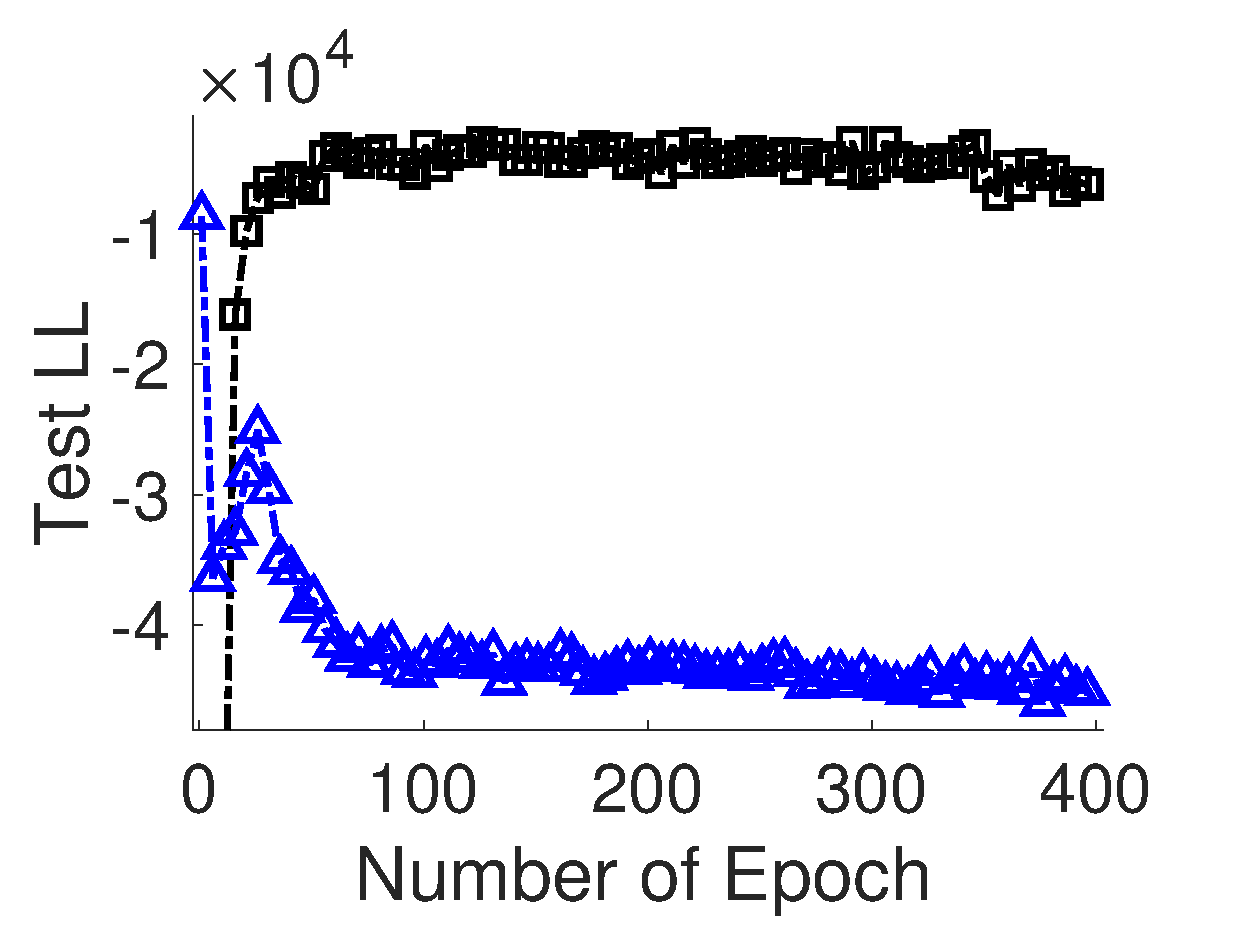
\includegraphics[width=\linewidth]{./figs/ufo_ll_epoch.eps}
			\caption{\textit{UFO}}
		\end{subfigure} 
		&
		\begin{subfigure}[t]{0.48\linewidth}
			\centering
			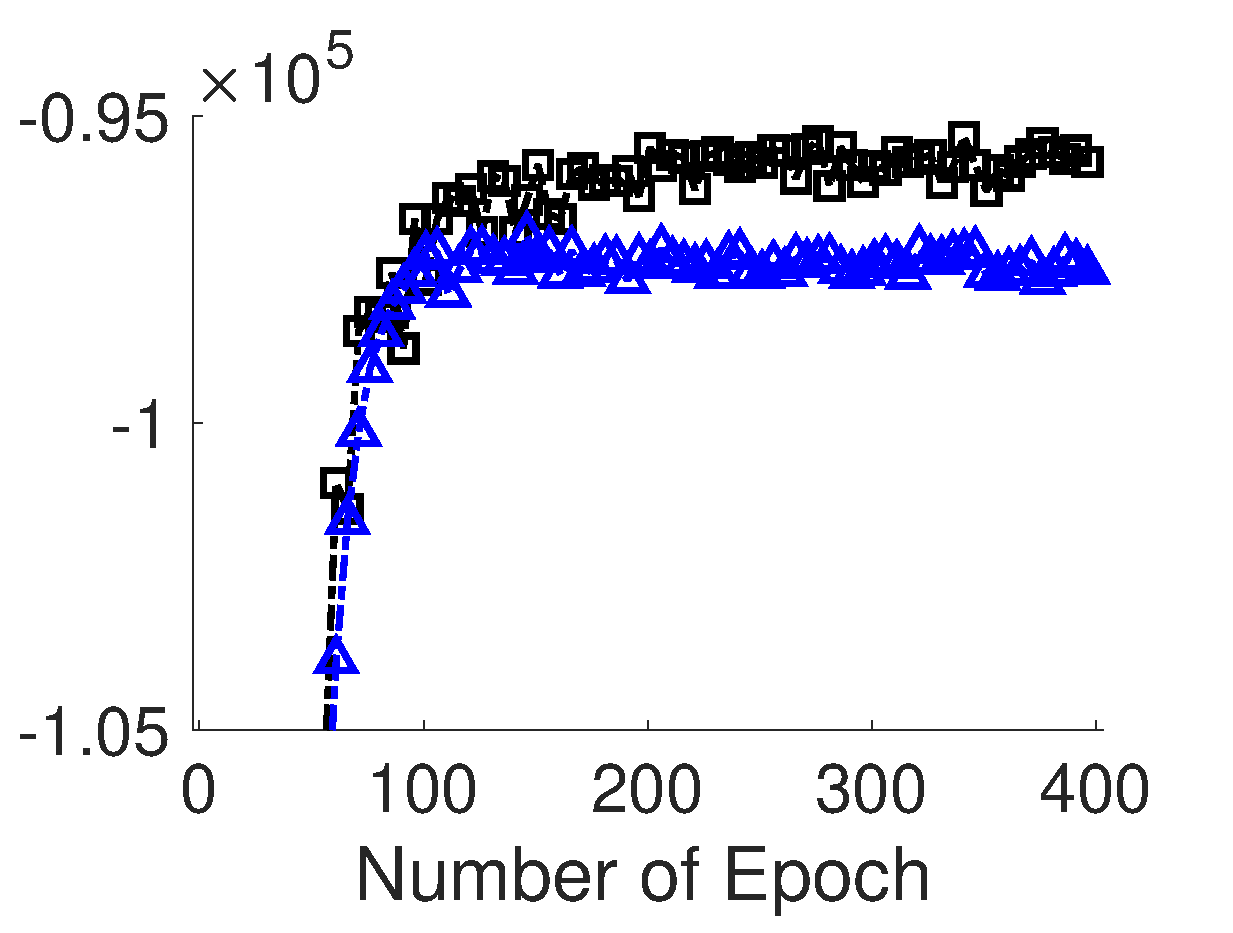
\includegraphics[width=\linewidth]{./figs/crash_ll_epoch.eps}
			\caption{\textit{Crash}}
		\end{subfigure}
	\end{tabular}
\vspace{-0.1in}
\caption{\small The test log likelihood of our method and HP-Local-50 along with the number of training epochs.} 	
\label{fig:learn-curve}
\vspace{-0.3in}
\end{figure}
\begin{figure*}
	\centering
	\setlength\tabcolsep{0.01pt}
	\begin{tabular}[c]{ccc}
		\raisebox{0.8in}{
			\begin{tabular}[c]{c}
				\begin{subfigure}[t]{0.23\textwidth}
					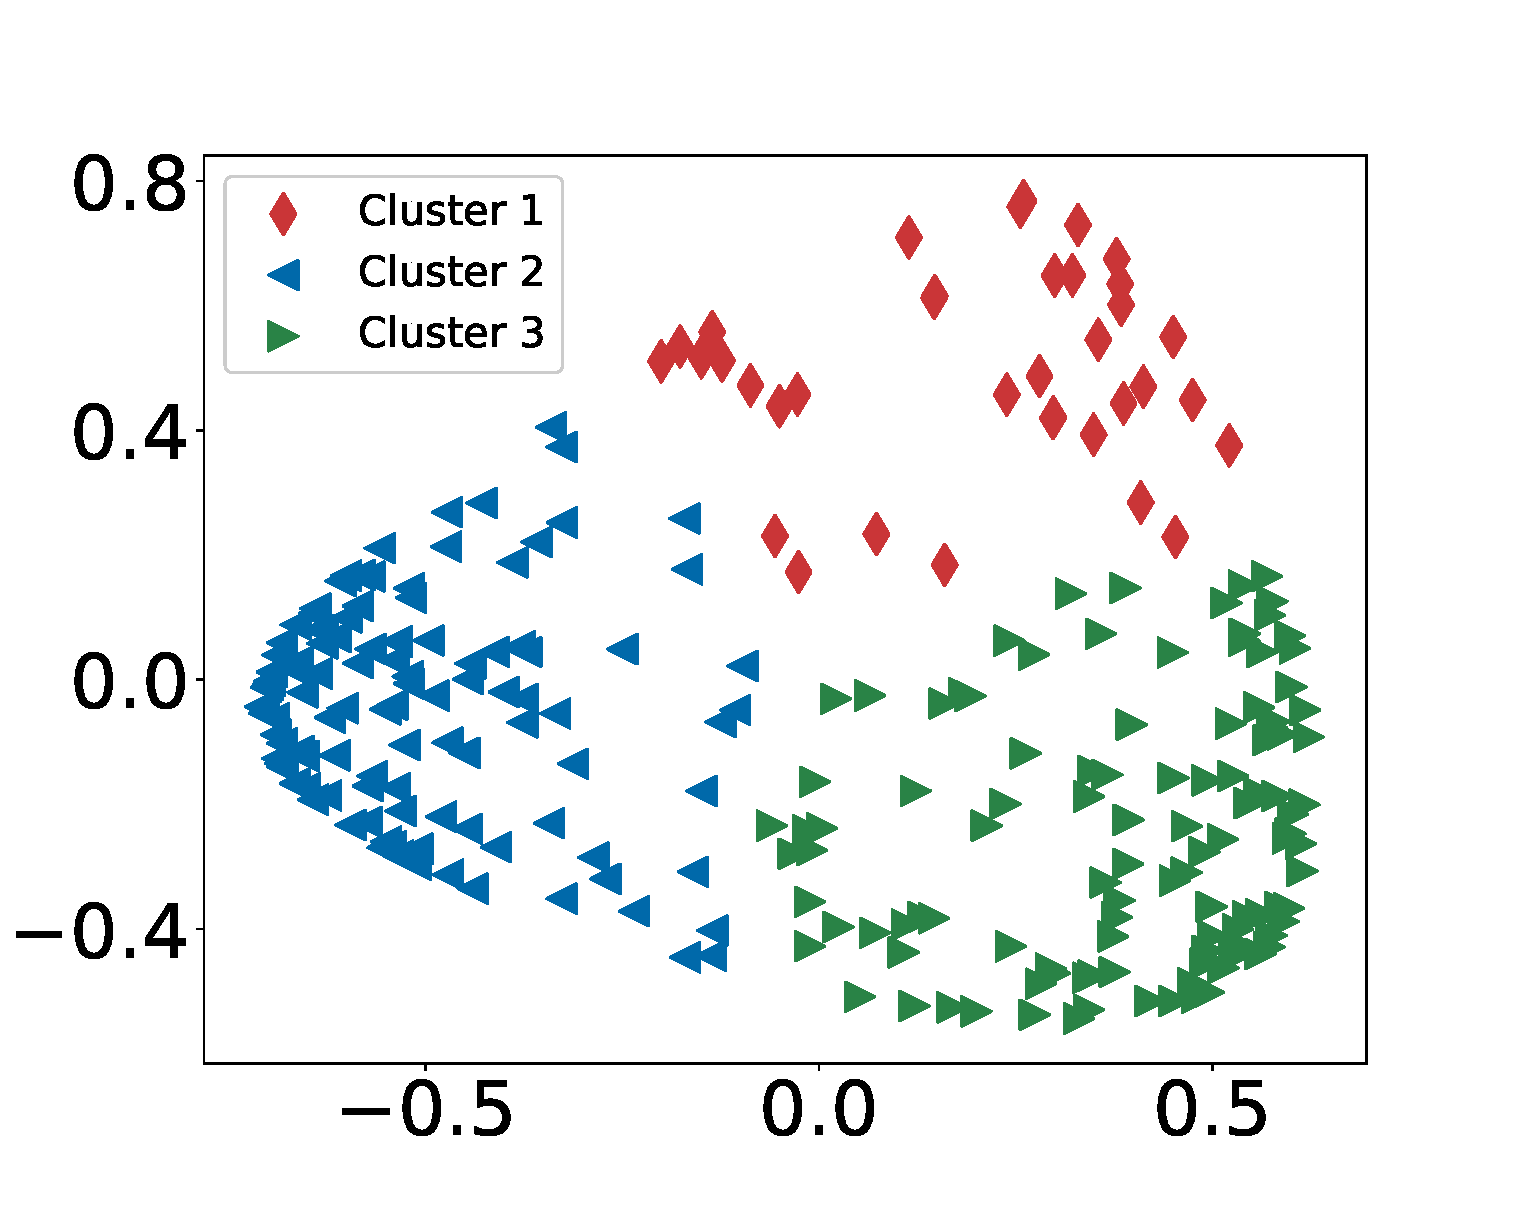
\includegraphics[width=\textwidth]{./figs/taobao_seller_cluster_scatter.eps}
					\caption{\textit{Sellers}}
				\end{subfigure}
				\\
				\begin{subfigure}[t]{0.23\textwidth}
					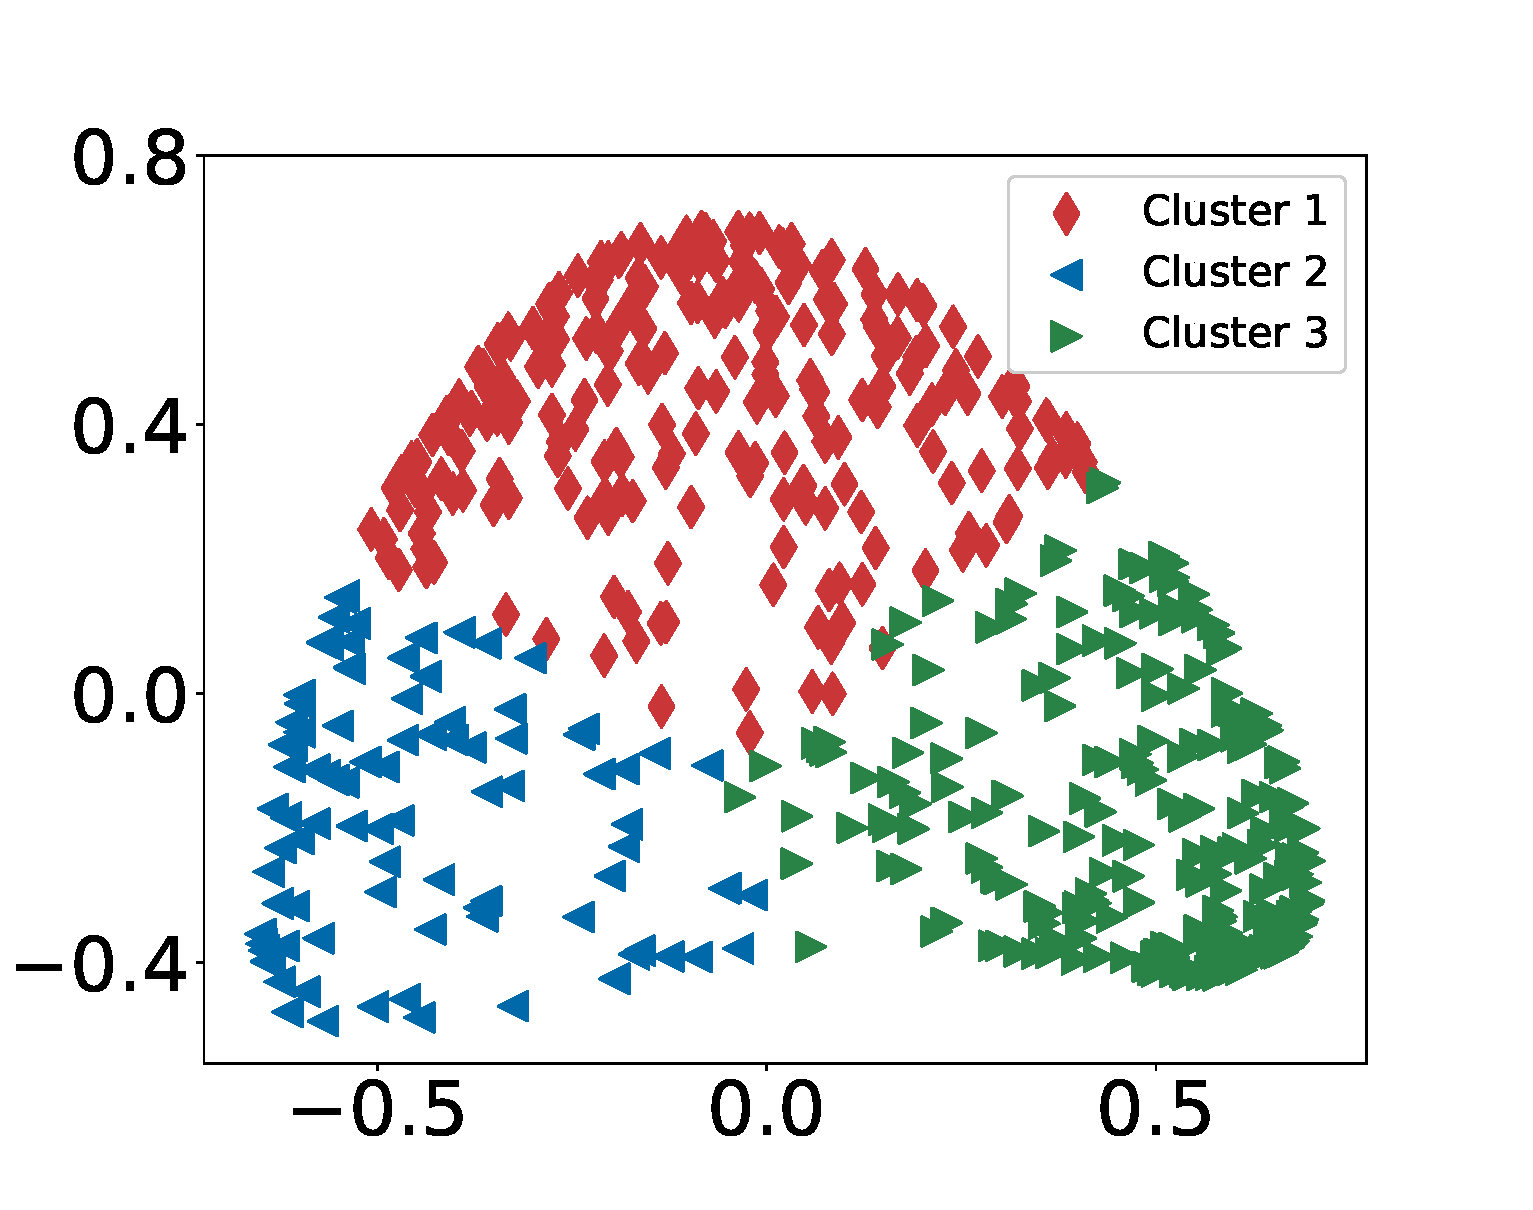
\includegraphics[width=\textwidth]{./figs/taobao_item_cluster_scatter.eps}
					\caption{\textit{Items}}
				\end{subfigure}
			\end{tabular} 
		} &
		\raisebox{0.8in}{
			\begin{tabular}[c]{c}
				\begin{subfigure}[t]{0.23\textwidth}
					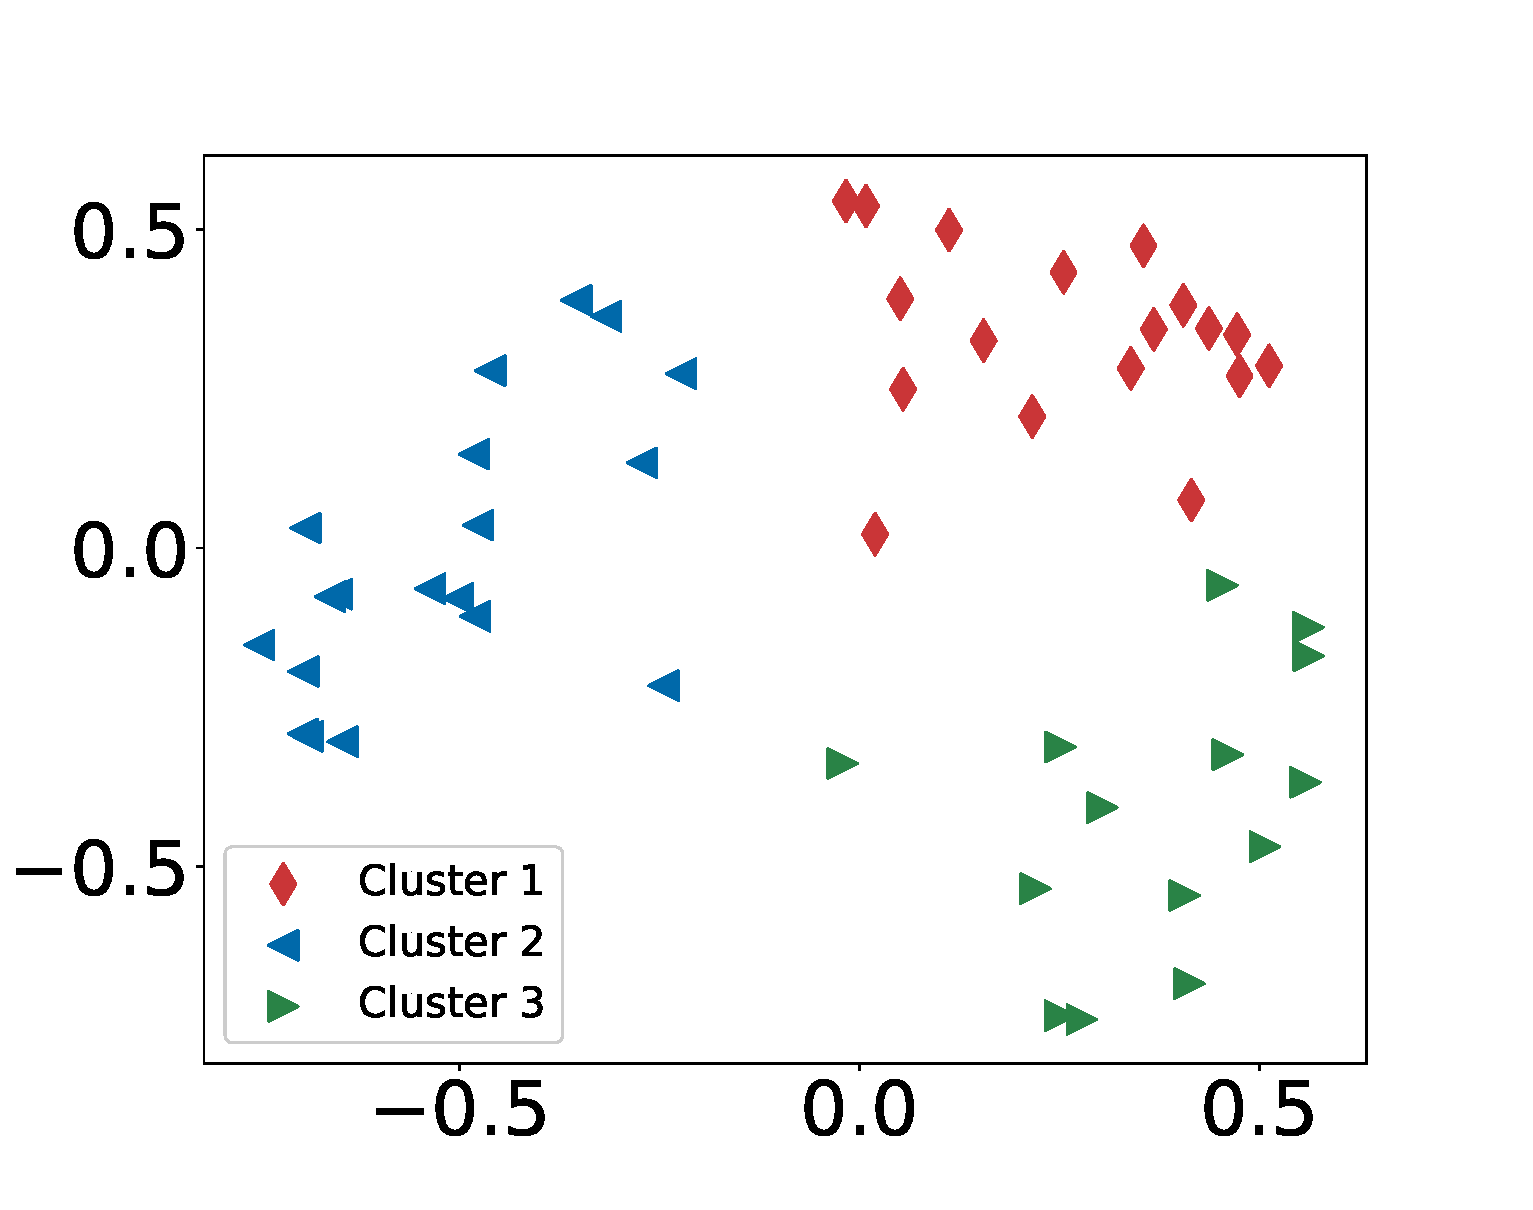
\includegraphics[width=\textwidth]{./figs/SMIE-structure/crash_state_cluster_scatter.eps}
					\caption{\textit{States}}
				\end{subfigure}
				\\
				\begin{subfigure}[t]{0.23\textwidth}
					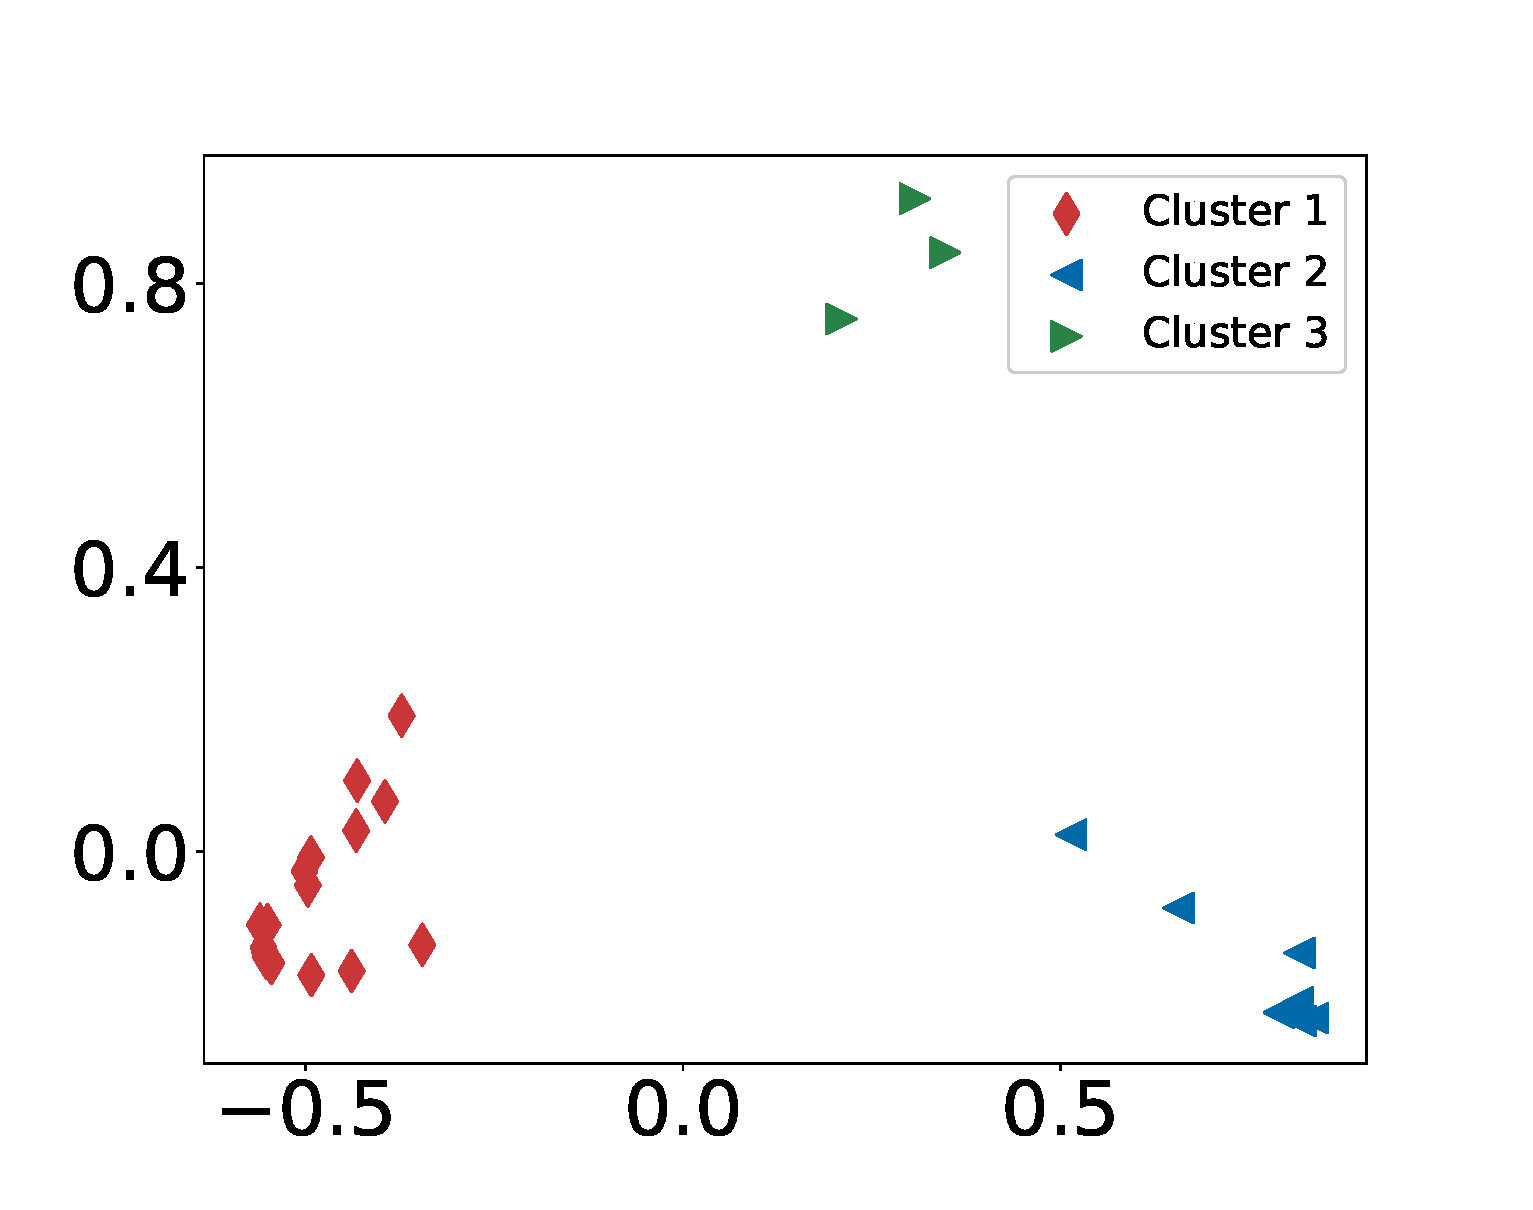
\includegraphics[width=\textwidth]{./figs/ufo_shape_cluster_scatter.eps}
					\caption{\textit{UFO shapes}}
				\end{subfigure}
			\end{tabular} 
		}
		&
		\begin{subfigure}[t]{0.4\textwidth}
			\centering
			\includegraphics[width=\textwidth]{./figs/SMIE-structure/crash-2015-state-trim.pdf}
			\caption{Geolocations of the state clusters}
		\end{subfigure}
	\end{tabular}
\vspace{-0.15in}
	\caption{\small Structures reflected from the latent factors learned by our model on \textit{Taobao} (a, b), \textit{Crash} (c, e) and \textit{UFO} (d). Colors indicate cluster memberships.}\label{fig:crash-ufo}
	\vspace{-0.2in}
\end{figure*}
\textbf{Results.} As we can see from Fig. \ref{fig:test-ll}, our approach consistently outperforms all the competing method except that on \textit{LastFM}, our method is a bit worse than HP-Local when the number of latent factors is $2$. The results demonstrate the advantage of our method in terms of predictive performance. Note that in general, when we increased the window size, HP-Local obtained better or similar prediction accuracy (\eg Fig. \ref{fig:test-ll}a); hence it  shows that estimating long-range temporal dependencies can help improve the predictive performance.  The other competing methods, \eg CP-PTF, GP-PTF, CP-NPTF and GP-NPTF, are far worse than our model and HP-Local in almost all the cases. For better illustration, we show their test log likelihoods in separate sub-figures at the bottom.  Note that these methods are based on homogeneous or non-homogeneous Poisson processes and disregard the temporal dependencies among the interaction events. Therefore, their results further demonstrate the benefit of our model being capable of capturing various, complex temporal dependencies among the events. 


We then investigated the learning behaviour of our model, as shown in Fig. \ref{fig:learn-curve}. Our learning algorithm converges reasonably fast (around $100$ epochs on both \textit{UFO} and \textit{Crash}), and then keeps stable after the convergence. Hence, there is not an apparent overfitting issue and we do not need to use extra tricks such as early stopping. The reason might be that our training objective \eqref{eq:elbo-3} is a lower bound of the model evidence and can effectively resist overfitting (like many other variational inference algorithms). 
\begin{figure}
	\vspace{-0.1in}
	\centering
	\setlength\tabcolsep{0.01pt}
	\begin{tabular}[c]{cc}
		\begin{subfigure}[t]{0.23\textwidth}
			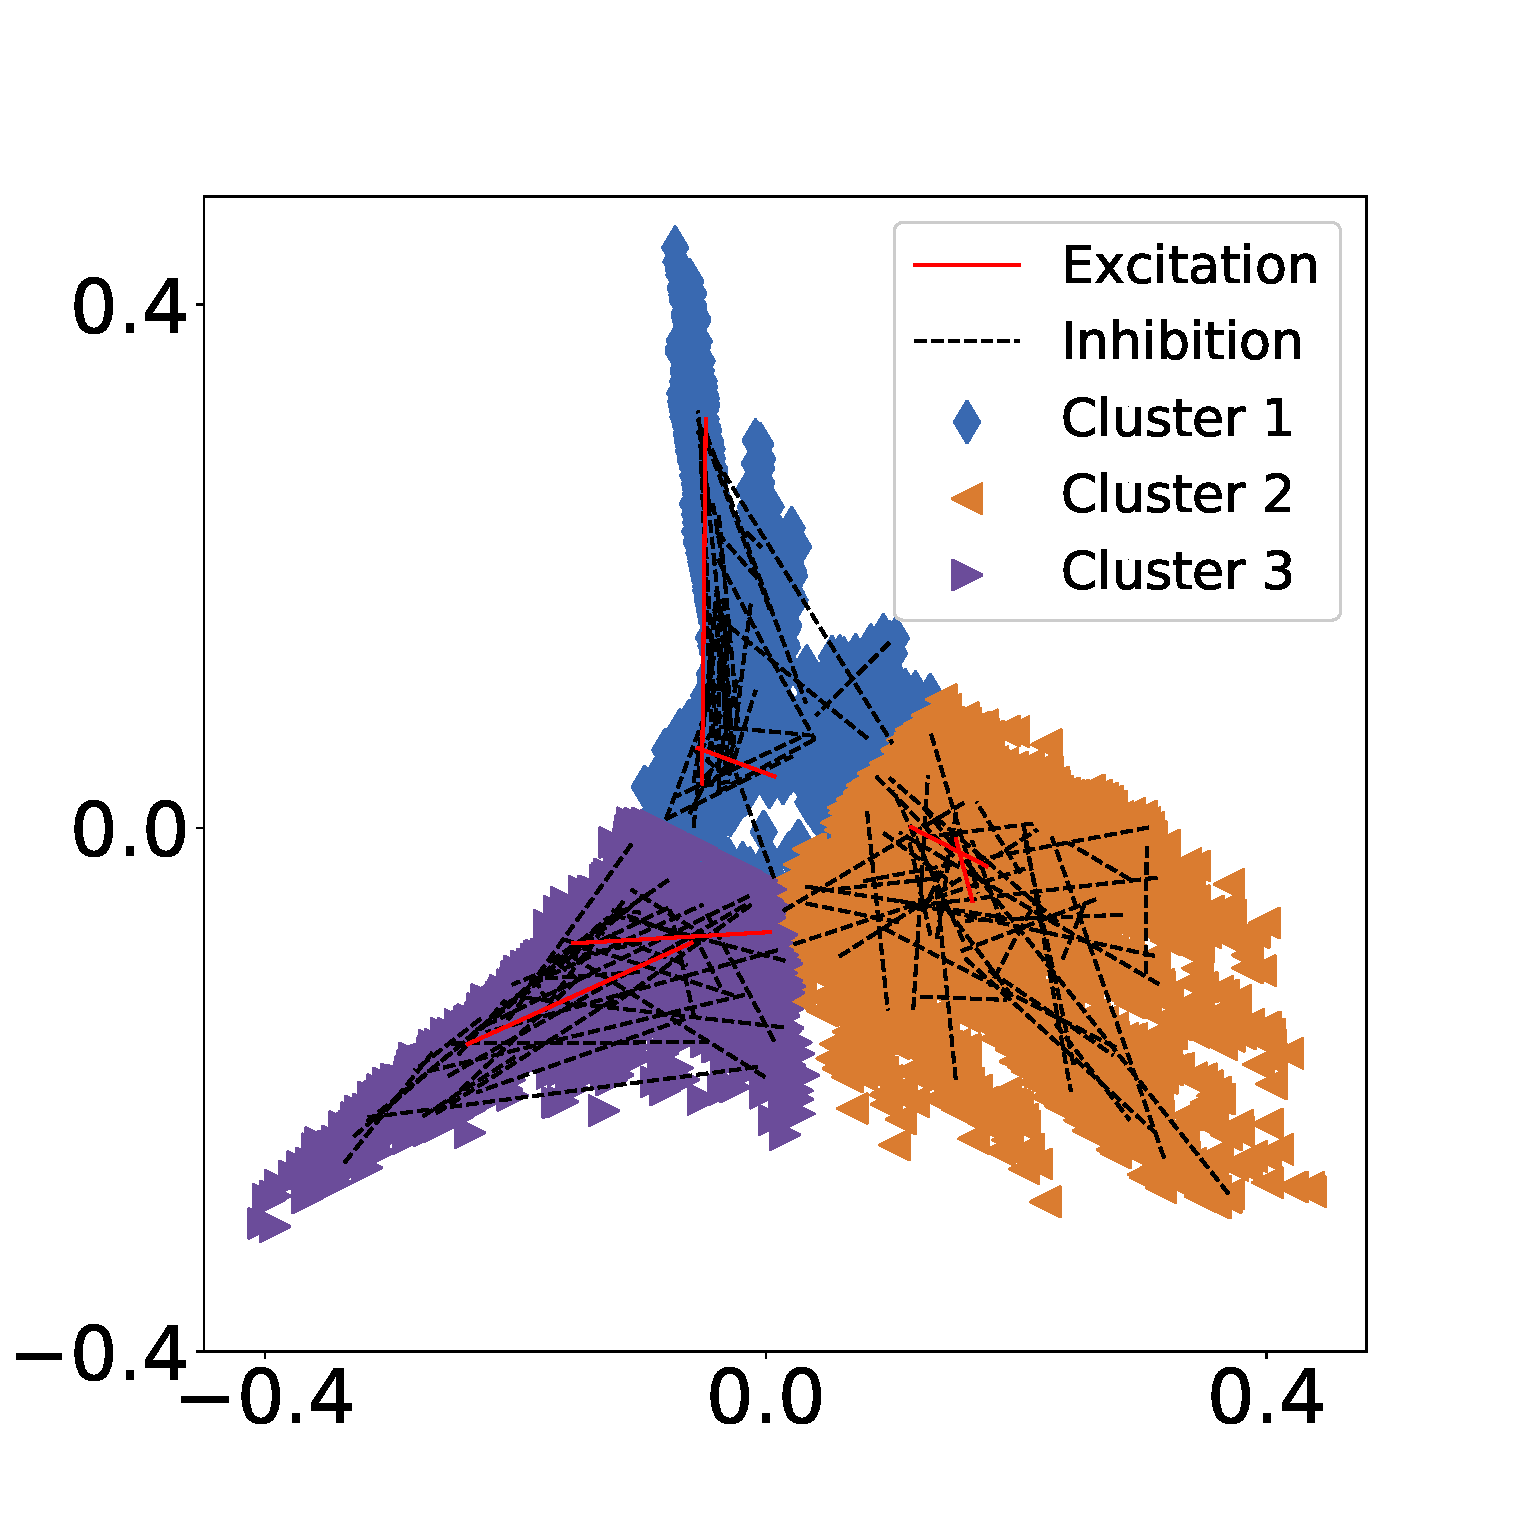
\includegraphics[width=\textwidth]{./figs/lastfm_s3_inner.eps}
			\caption{\textit{Within clusters}}
		\end{subfigure} &
		\begin{subfigure}[t]{0.23\textwidth}
			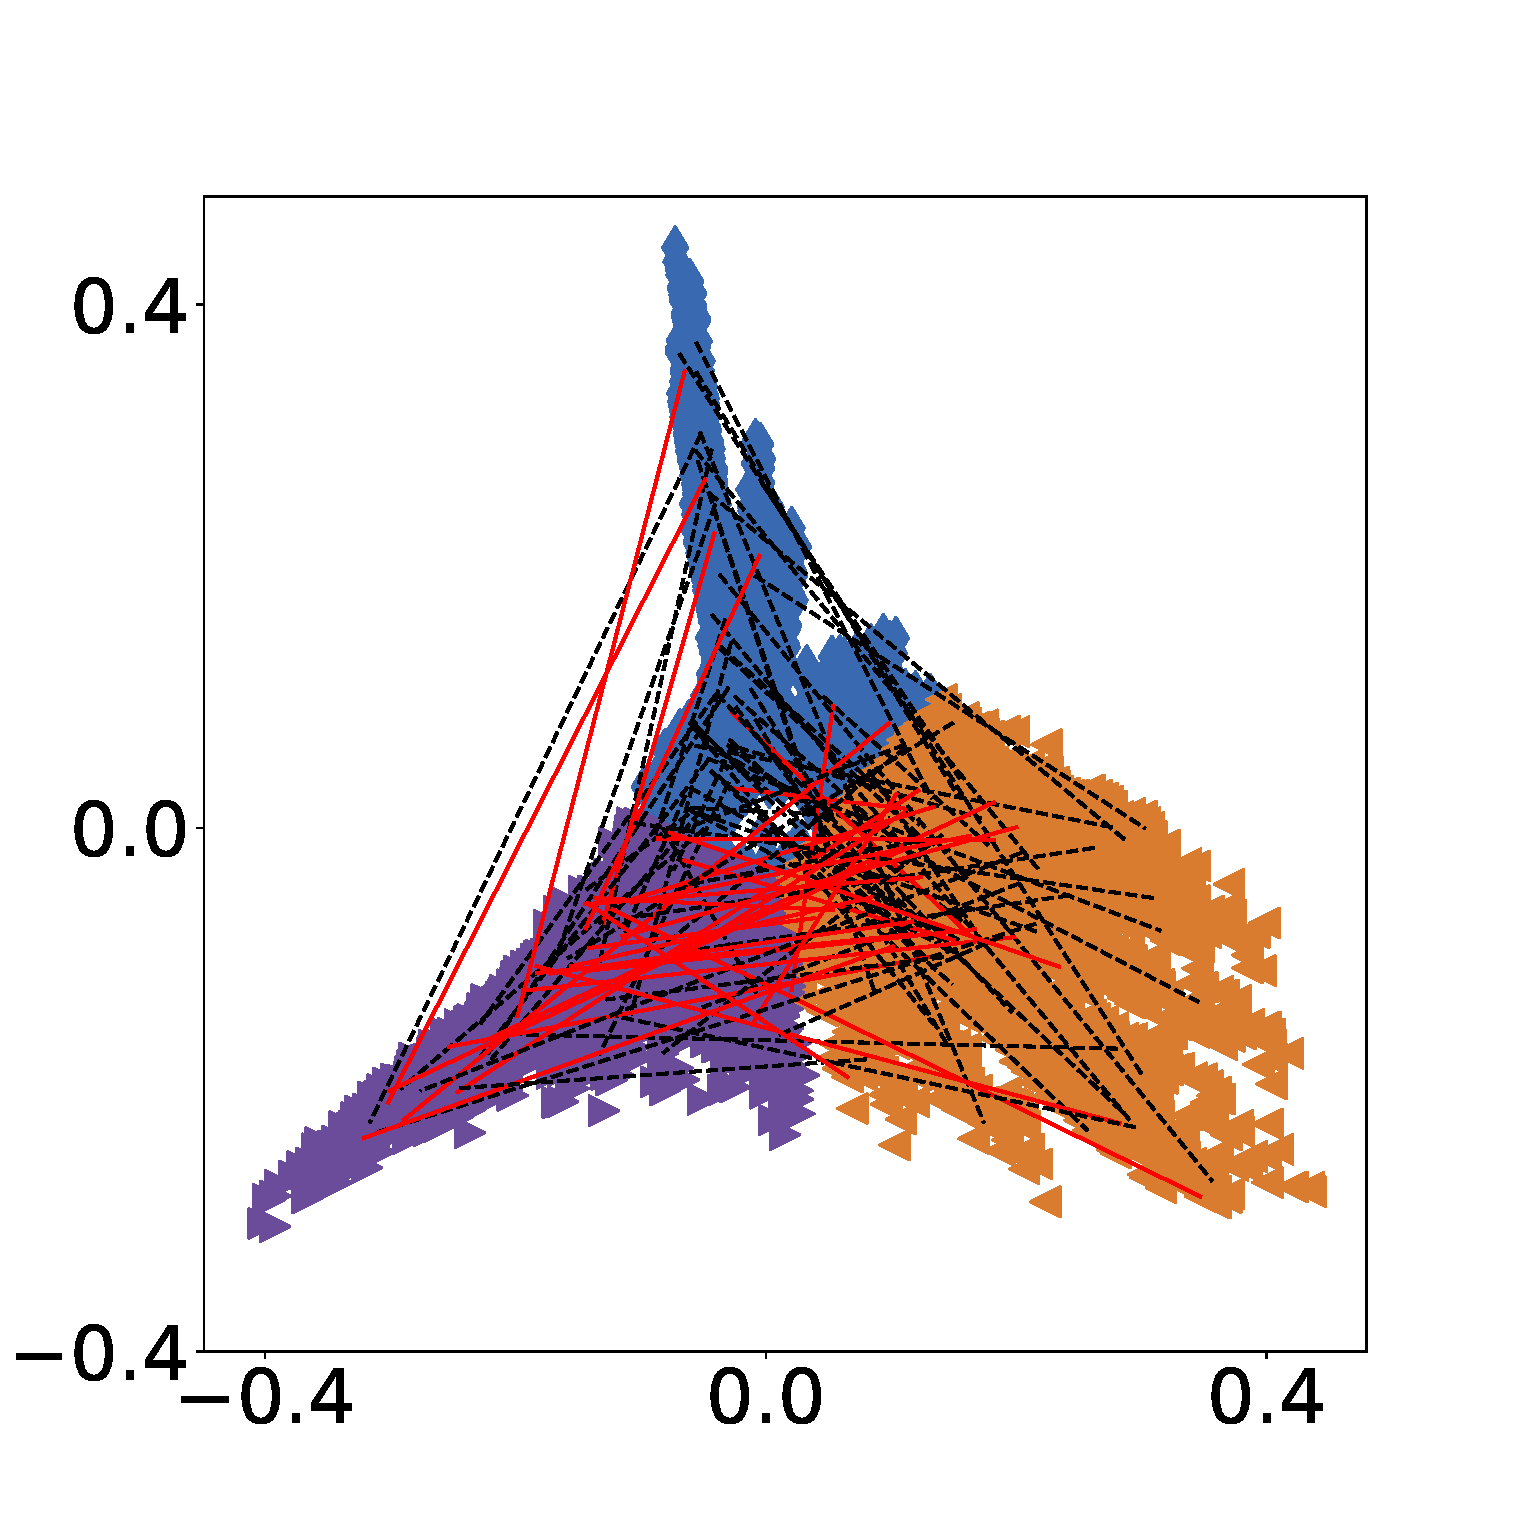
\includegraphics[width=\textwidth]{./figs/lastfm_s3_cross.eps}
			\caption{\textit{Across clusters}}
		\end{subfigure}
	\end{tabular}
\vspace{-0.15in}
	\caption{\small Structures of the events and their temporal influences in \textit{LastFM}.} \label{fig:lastfm} 
	\vspace{-0.3in} 
\end{figure}
\vspace{-0.1in}
\subsection{Structure Discovery}
\vspace{-0.05in}
Next, we examined if our method can discover hidden structures in the data. To this end, we set the number of latent factors to $10$ and ran our algorithm on \textit{Crash}, \textit{UFO} and \textit{Taobao}. Then we applied kernel PCA~\citep{scholkopf1998nonlinear} (with RBF kernel) to project the latent factors onto the x-y plane. We then ran k-means to find the potential clusters in the (projected) factor representations of the entities. We used the elbow method~\citep{ketchen1996application} to select the number of clusters. As we can see from Fig. \ref{fig:crash-ufo}, these factors reflected clear grouping structures. Note that \textit{Taobao} data have been anonymized so we cannot investigate the meaning of those clusters. But they can be potentially useful for tasks like recommendation~\citep{tran2018regularizing} and click-through-rate prediction~\citep{pan2019warm}. Then for \textit{Crash} data, we show the actual geolocations of the clustered states in Figure \ref{fig:crash-ufo}e. We can see that states grouped together are often neighbouring with each other. The clusters can be roughly seen as the middle (red), the south (blue) and the east/west coast (green). This is reasonable --- the states close by may have similar patterns of the traffic crash events and their chain effects (inhibition/excitation) due to similar driving customs, roads layout and weather patterns. 

We also looked into the triggering and inhibition effects among the interaction evens. To this end, we ran our algorithm on \textit{LastFM}. We represented each music tagging event by concatenating the latent factors of participants, \ie the user, artist and tag. We then used kernel PCA to project the event representations onto the x-y plane, and ran k-means to obtain the clusters. We then randomly sample pairs of events within and across clusters, and show their triggering/inhibition relationships with red/black colors. As shown in Fig. \ref{fig:lastfm}a and b, the factor representations of the events present a clear cluster structure. Interestingly, we can see that events within the same cluster mainly inhibit each other (see Fig. \ref{fig:lastfm}a), while across different clusters often excite each other (see Fig. \ref{fig:lastfm}b). This might because users tend to tag artists with distinct/orthogonal styles, rather than keep tagging the same types of artists with very close tags/labels. 

